\documentclass[draft]{article}

\usepackage{amsmath,amssymb,amsthm,mathtools}
\usepackage[linesnumbered, ruled]{algorithm2e}
\usepackage[]{subfig}
\usepackage{paralist}
\usepackage{hyperref}
\hypersetup{final}
\usepackage[inline]{enumitem}

% DEBUG
\usepackage{fullpage}
\usepackage{todonotes}
\usepackage{lineno}
\linenumbers

% EXTRA
\usepackage{authblk}
\def\CARPOOL{maximum carpool matching}

\newcommand{\din}[1][M]{deg^{#1}_{in}}
\newcommand{\dout}[1][M]{deg^{#1}_{out}}
\newcommand{\dinout}[1][M]{deg^{#1}}

\DeclareMathOperator*{\argmin}{arg\,min}
\DeclareMathOperator*{\argmax}{arg\,max}

\def\R{\mathbb{R}}
\def\N{\mathbb{N}}

\newtheorem{observation}{Observation}
\newtheorem{lemma}{Lemma}
\newtheorem{theorem}{Theorem}
\newtheorem{definition}{Definition}
\newtheorem{remark}{Remark}
\usepackage{tikz}
\usetikzlibrary{
	arrows,
	arrows.meta,
	calc,
	graphs,
	patterns,
	positioning,
	shapes,
	decorations.pathmorphing,
}

%DEFAULT STYLE
\tikzset{default style/.style={
	>=Stealth, 
	on grid, 
	auto, 
	thick,
}}

% NODE
\tikzset{default node/.style={
	draw, 
	circle,
	inner sep=0mm,
	minimum size=5mm,
	very thick,
	font=\small,
	black!70,
}}

% LABELS
\tikzset{label/.style={
	draw=none,
	sloped,
}}

\tikzset{label above/.style={
	label,
	midway,
	above=-1mm,
}}

\tikzset{label below/.style={
	label,
	midway,
	below=-1mm,
}}

\title{Improved Approximation Algorithms for the Maximum Carpool Matching
Problme}

\date{}
\author[1]{Reuven Bar-Yehuda	\thanks{\texttt{reuven@cs.technion.ac.il}}}
\author[1]{Gilad Kutiel			\thanks{\texttt{gkutiel@cs.technion.ac.il}}}
\author[2]{Dror Rawitz			\thanks{\texttt{dror.rawitz@biu.ac.il}}}

\affil[1]{Department of Computer Science, Technion, Haifa, Israel}
\affil[2]{Faculty of Engineering, Bar Ilan University, Ramt-Gan, Israel}

\begin{document}
\maketitle

\begin{abstract}
The \textsc{\CARPOOL{}} problem is a star packing problem in directed graphs.
Formally, given a directed graph $G = (V, A)$,
a capacity function $ c: V \rightarrow \N $,
and a weight function $w : A \rightarrow \R $,
a feasible \emph{carpool matching} is a triple 
$(P, D, M)$, where $P$ (passengers) and $D$ (drivers) form a partition of $V$, 
and $M$ is a subset of $A \cap (P \times D)$,
under the constraints that for every vertex $d \in D$, 
$\din(d) \leq c(d)$, 
and for every vertex $p \in P$, $\dout(p) \leq 1$.
In the \textsc{\CARPOOL{}} problem we seek for a matching $(P, D, M)$ that maximizes the
total weight of $M$.

The problem arises when designing an online carpool service, 
such as Zimride~\cite{zimride}, 
that tries to connect between passengers and drivers based on (arbitrary) similarity function.
The problem is known to be NP-hard, 
even for uniform weights and without capacity constraints.

we show that the problem can be formulated as
unconstarints submodular maximization problem, 
thus it has a $\frac{1}{2}$-approximation algorithm.
For the unweighted variant of the problem when the maximum possible capacity, $C$, is
fixed, we give a $(\frac{C + 1}{2C} - \varepsilon)$-approximation algorithm
for the any $\varepsilon > 0$.
\end{abstract}

\section{Introduction}
Carpooling, is the sharing of car journeys so that more than one person travels
in a car.
Knapen et al.~\cite{knapen2013estimating} describe an automatic service
to match commuting trips.
Users of the service register their personal profile and a set of periodically
recurring trips, 
and the service advises registered candidates on how to combine their commuting
trips by carpooling.
The service acts in two phases. 

In the first phase, the service estimates the probability that a person $a$
traveling in person's $b$ car will be satisfied by the trip.
This is done based on personal information and feedback from users on past
rides.
The second phase is about finding a carpool matching
that maximizes the global (total expected) satisfaction.

The second phase can be modeled in terms of graph theory.
Given a directed graph $G = (V, A)$.
Each vertex $v \in V$ corresponds to a user of the service and an arc
$(u, v)$ exists if the user corresponding to vertex $u$ is willing to
commute with the user corresponding to vertex $v$.
A capacity function $ c: V \rightarrow \N $ is defined
according to the number of passengers each user can drive if she was
selected as a driver.
A weight function $w : A \rightarrow \R $ defines the amount of
satisfaction $w(u, v)$,
that user $u$ gains when riding with user $v$.

A feasible \emph{carpool matching} (matching) is a triple 
$(P, D, M)$, where $P$ and $D$ form a partition of $V$, 
and $M$ is a subset of $A \cap (P \times D)$,
under the constraints that for every driver $d \in D$, 
$\din(d) \leq c(d)$, 
and for every passenger $p \in P$, ${\dout(p) \leq 1}$.
In the \textsc{\CARPOOL{}} problem we seek for a matching $(P, D, M)$ that maximizes the
total weight of $M$.
In other words, the \textsc{\CARPOOL{}} problem is about finding a set of 
(directed toward the center) vertex disjoint stars 
that maximizes the total weights on the arcs.
Figure~\ref{fig:carpool} is an example of the \textsc{\CARPOOL{}} problem.

\begin{figure}
\centering
\newcommand{\edge}[3]{
	\draw (#1) -- (#2) node[label above] {#3};
}
\subfloat[]{
\label{subfloat:input}
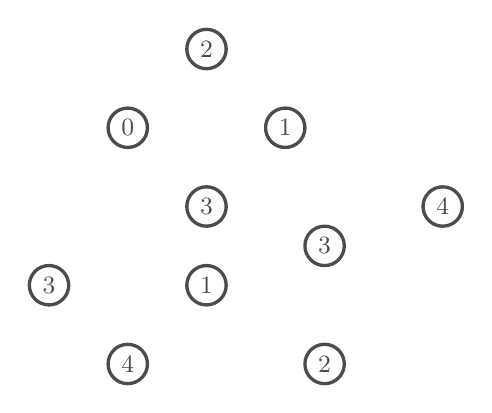
\begin{tikzpicture}[every node/.style={default node}, ->, very thick]

\node(1) at(-1,3) {2};
\node(2) at(.5,.5) {3};
\node(3) at(-1,0) {1};
\node(4) at(-1,1) {3};
\node(5) at(-2,2) {0};
\node(6) at(-2,-1) {4};
\node(7) at(-3,0) {3};
\node(8) at(.5,-1) {2};
\node(9) at(0,2) {1};
\node(10) at(2,1) {4};

\edge{1}{4}{3}
\edge{2}{4}{4}
\edge{3}{4}{5}

\edge{5}{7}{2}
\edge{6}{7}{4}

\edge{8}{10}{6}
\edge{9}{10}{2}

\edge{1}{5}{4}
\edge{4}{5}{4}

\edge{2}{3}{2}
\edge{6}{3}{2}
\edge{7}{3}{2}

\edge{8}{2}{1}
\edge{10}{2}{1}

\edge{3}{8}{3}
\edge{8}{3}{3}

\edge{1}{9}{1}
\edge{4}{9}{1}

\end{tikzpicture}}
\hfill\subfloat[]{
\label{subfloat:output}
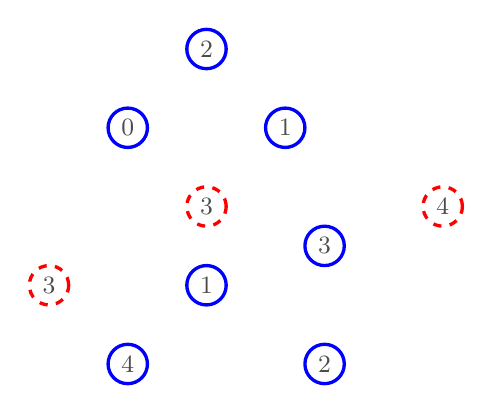
\begin{tikzpicture}[every node/.style={default node}, ->, very thick]

\begin{scope}[every node/.style={default node, draw=blue}]
\node(5) at(-2,2) {0};
\node(6) at(-2,-1) {4};

\node(2) at(.5,.5) {3};
\node(3) at(-1,0) {1};
\node(1) at(-1,3) {2};

\node(8) at(.5,-1) {2};
\node(9) at(0,2) {1};
\end{scope}

\begin{scope}[every node/.style={default node, draw=red, dashed}]
\node(7) at(-3,0) {3};

\node(4) at(-1,1) {3};

\node(10) at(2,1) {4};
\end{scope}


\edge{1}{4}{3}
\edge{2}{4}{4}
\edge{3}{4}{5}

\edge{5}{7}{2}
\edge{6}{7}{4}

\edge{8}{10}{6}
\edge{9}{10}{2}

\end{tikzpicture}}
\caption[]{
\label{fig:carpool}
A carpool matching example: 
\subref{subfloat:input} 
a directed graph with capacities on the vertices and weights on the arcs. 
\subref{subfloat:output}
a feasible matching with total weight of 26.
$P$ is the set of blue vertices, and $D$ is the set of red, dashed vertices. 
}
\end{figure}  

Hartman et al.~\cite{hartman2013optimal} proved that the
\emph{\CARPOOL{}} problem considered in this paper is NP-hard,
and that the problem remains NP-hard even for a binary weight function when
the capacity function $c(v) \leq 2$ for every vertex in $V$.
It is also worth mentioning, that in the undirected, uncapacitated, unweighted
variant of the problem, the set of drivers in an optimal solution
form a minimum dominating set.
When the set of drivers is known in advanced, however, the problem becomes
tractable and can be solved using a reduction to a flow network problem.

Agatz et al.~\cite{agatz2012optimization} outlined the optimization challenges
that arise when developing technology to support ride-sharing and survey the
related operations research models in the academic literature.  
Hartman et al.~\cite{hartman2014theory} designed several heuristic algorithms
for the \CARPOOL{} problem and compared 
their performance on real data.
Other heuristic algorithms were developed as well~\cite{knapen2014exploiting}.
Arkin et al.~\cite{arkin2004approximations}, considered other variants of
capacitated star packing where a capacity vector is given as part of the input and 
capacities need to be assigned to vertices.  

Nguyen et al.~\cite{nguyen2008approximating} considered the \textsc{spanning star forest} problem
(the undirected, uncapacitated, unweighted variant of the problem).
They proved the following results:
\begin{enumerate*}
\item
there is a polynomial-time approximation scheme for planner graphs;
\item 
there is a polynomial-time $\frac{3}{5}$-approximation algorithm for graphs;
\item 
there is a polynomial-time $\frac{1}{2}$-approximation algorithm for weighted graphs.
\end{enumerate*}
They also showed how to apply the spanning star forest model to aligning multiple
genomic sequences over a tandem duplication region.
Chen et al.~\cite{chen2007improved} improved the approximation ratio to 0.71,
and also showed that the problem can not be approximated to within a factor of
$\frac{31}{32} + \epsilon$ for any $\epsilon > 0$ under the assumption 
that $\text{P} \neq \text{NP}$.
It is not clear, however, if any of the technique used to address the
\textsc{spanning star forest} problem can be generalized to approximate the
directed capacitated variant.

In section~\ref{sec:sub} we show that the problem can be formulated as
unconstarints submodular maximization problem, thus it has a 2-approximation
algorithm.
In section~\ref{sec:local} we consider the unweighted variant of the problem.
We show that when the maximum possible capacity, $C$, is fixed, there is a 
$(\frac{C + 1}{2C} - \varepsilon)$-approximation algorithm for the any $\varepsilon > 0$.

\section{Submodularity}
\label{sec:sub}
In this section we show that the problem can be formulated as unconstrained
submodular maximization problem, and thus, it has a 2-approximation algorithm.

Consider the function $w : 2^V \to \R$ where $w(D)$ is the value of the optimal
carpool matching when the set of drivers is $D$.
As we mention in the introduction, $w$ can be computed efficiently.

\begin{theorem}
$w$ is submodular.
\end{theorem}

\begin{proof}
Consider two subsets $A,B \subseteq V$, 
we need to show that $w(A) + w(B) \geq w(A \cup B) + w(A \cap B)$.
Let $E_{A \setminus B} = (V \setminus A) \times (A \setminus B)$, 
$E_{B \setminus A} = (V \setminus A) \times (B \setminus A)$,
and $E_{B \cap A} = (V \setminus (A \cap B)) \times (B \cap A)$.
 
Let $M_{A \cup B}$ and $M_{A \cap B}$ be the set of edges in an optimal
matching when the set of drivers are $A \cup B$ and $A \cap B$ respectively.
We argue that we can construct two (feasible) matchings $M_A$ and $M_B$ using
the sets of drivers $A$ and $B$ respectively and 
$w(M_A) + w(M_B) = w(M_{A \cup B}) + w(M_{A \cap B})$.
First, take all the edges from $M_{A \cup B} \cap E_{A \setminus B}$ and 
add them to $M_A$, 
add $M_{A \cup B} \cap E_{B \setminus A}$ to $M_B$.
Clearly this can be done.
Now, split the edges from $M_{A \cap B} \cup (M_{A \cup B} \cap E_{A \cap B})$
between $M_A$ and $M_B$ in a way that does not violate the capacity constraints.
One can verify that this can be done.
\end{proof}

\section{Constant Max Capacity}
In this section we study the carpool problem when the maximum possible capacity
is constant.
We show that this variant of the problem is APX-hard as well.
We also describe and analyze a local search algorithm for the unweighted
variant of the problem, 
and show that the algorithm achieves a 
$\frac{C + 1}{2C} - \varepsilon$ approximation ratio for any $\varepsilon > 0$.
Throughout this section we consider $C$ to be fixed, and $k$ to be a fixed parameter.  

	\subsection{Hardness}
	\label{sec:hardness}
As we mentioned in the introduction, the maximum spanning star forest can not 
be approximated within a factor of 
$\frac{31}{32} + \epsilon$ for any $\epsilon > 0$ unless P = NP.
The proof, however, does not hold for the case when the maximum capacity is
constant. 
In this subsection we show that the problem remains APX-hard even in this case.

Formally, the (unweighted)
minimum dominating set problem is defined as $\min_{D}(|D|)$,
where $D$ is any feasible dominating set.
It is also easy to see that the (unweighted, undirected, uncapacitated) 
maximum carpool matching problem can be defined as $max_{D}(|V \setminus D|)$, 
where $D$ is any feasible dominating set.
The \textsc{Dominating Set-B} is the problem of finding minimum dominating set on 
graphs with degree bounded by $B$,
and it was shown to be APX-hard (for $B \geq 3$) by 
Papadimitriou et al.~\cite{papadimitriou1988optimization}.

Let $G$ be a b-bounded degree graph,
let $D^*(G)$ be a minimum dominating set in $G$,
and let $C^*(G)$ be a maximum carpool matching in $G$, 
then the following lemmas hold:

\begin{lemma}
$|C^*| = |V| - |D^*|$
\end{lemma}

\begin{proof}
The proof follows immediately from the definitions of the two problems. 
\end{proof}

\begin{lemma}
\label{lm:optc_leq_boptd}
$|C^*| \leq b \cdot |D^*|$
\end{lemma}

\begin{proof}
The proof follows directly from the observation that $|D^*| \geq \frac{|V|}{b}$.
\end{proof}

Let $C(G)$ be any feasible carpool matching on $G$, then the following lemma holds:

\begin{lemma}
\label{lm:erreq}
$|C^*| - |C| = (|V| - |C|) - |D^*|$
\end{lemma}

\begin{proof}
$$
|C^*| - |C| 				= 
|V| - |D^*| - |C| 	= 
(|V| - |C|) - |D^*|
$$
\end{proof}

Let $D(G)$ be any feasible dominating set in $G$, 
we argue that $f(G) = G$, and $g(C(G)) = V \setminus C(G)$ 
define a linear reduction (L-reduction) from the \textsc{Dominating Set-B} problem to the 
\textsc{\CARPOOL{}} problem.
\begin{proof}
By lemma~\ref{lm:optc_leq_boptd} we get that $C^*(f(G)) = C^*(G) \leq b \cdot D^*(G)$,
and by lemma~\ref{lm:erreq} we get that 
\begin{equation}
\begin{split}
|C^*(f(G))| - |C(G)|		& = |C^*(G)| - |C(G)| 			\\
							& = (|V| - |C(G)|) - |D^*(G)|	\\
							& = |g(C(G))| - |D^*(G)|
\end{split}
\end{equation}
\end{proof}

\begin{theorem}
The \textsc{\CARPOOL{}} problem is APX-hard.
\end{theorem}

\begin{proof}
The proof follows directly from the above linear reduction and the fact that 
\textsc{Dominating Set-B} is APX-hard. 
\end{proof}

	\subsection{Local Search}
	\label{sec:local}
The local search algorithm maintains a feasible matching throughout its execution
and operates in 
iterative manner where in each iteration it tries to find a better solution by
replacing a subset of the edges in the current solution with 
another (larger) subset of edges not in the solution.
The local search algorithm halts when no improvement can be done.
The algorithm is described in Algorithm~\ref{alg:local}. 

\begin{algorithm}
\SetKw{True}{true}
\SetKw{False}{false}
\KwIn{$G = (V, A)$, $c : V \rightarrow \N$, $k$}
\KwOut{$M$}
$M \leftarrow \emptyset$								\\
\Repeat{done}{
\label{line:outerloop}
 	$done \leftarrow{}$ \True							\\
 	\For{$M' \in M : |M'| \leq k$}{
 		\For{$A' \in A \setminus M : |A'| = |M'| + 1$}{
			\If{$M \setminus M' \cup A'$ is feasible}{
				$M \leftarrow{} M \setminus M' \cup A'$	\\
				$done \leftarrow{}$ \False				\\
			}
		}
 	}
}
\Return{$M$}

\caption{
\label{alg:local}
Local Search}
\end{algorithm}


We claim that the local search algorithm halts in polynomial time.
Observed that in every iteration the algorithm either improves the value of the solution
by one or otherwise it terminates. 
Thus, after a maximum of $n$ iterations the algorithm stops.
In every iteration we examine all the subsets of edges of a fixed size and test for feasibility,
both these operations can be done in polynomial time - $O(n^{Ck + 1})$. 

To analyze the approximation ratio achieved by the local search algorithm consider an 
arbitrary but fixed optimal matching $M^*$.
Given the solution outputted by the local search algorithm, 
$M$, 
we build the \emph{star graph} of the two solutions
in which each node represents a star from the optimal solution 
and edges exits between two nodes if
there is a star in $S(M)$ that intersect the two
corresponding stars of the optimal solution, 
formally $G^{M^*}_M = (S, E)$ where $\{v_i : S^*_i \in S(M^*) \}$ 
and 
$E = \{(v_i, v_j) : 
\exists S \in M,
S \cap S^*_i \neq \emptyset \land S \cap S^*_j \neq \emptyset,
\}$.
Figure~\ref{fig:conflict} depicts a star graph.

\begin{figure}[ht]
\centering
\subfloat[]{
\label{subfloat:graph}
\newcommand{\edge}[2]{
	\draw (#1) -- (#2);
}

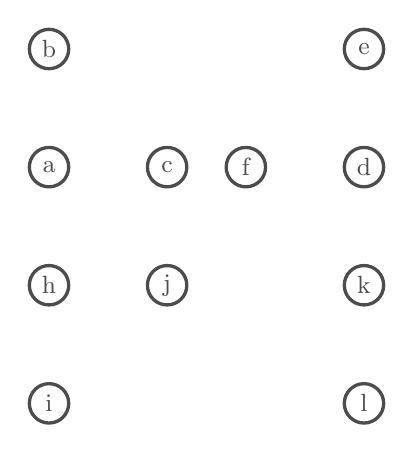
\begin{tikzpicture}[every node/.style={default node}, ->, very thick]

\node(1) at(0,0) {a};
\node(2) at(0,1.5) {b};
\node(3) at(1.5,0) {c};

\node(4) at(4,0) {d};
\node(5) at(4,1.5) {e};
\node(6) at(2.5,0) {f};

\node(7) at(0,-1.5) {h};
\node(8) at(0,-3) {i};
\node(9) at(1.5,-1.5) {j};

\node(10) at(4,-1.5) {k};
\node(11) at(4,-3) {l};

\begin{scope}[dashed, red]
\edge{2}{1}
\edge{3}{1}

\edge{5}{4}
\edge{6}{4}

\edge{8}{7}
\edge{9}{7}

\edge{11}{10}
\end{scope}

\begin{scope}[green]
\edge{2}{5}

\edge{7}{1}
\edge{3}{9}
\end{scope}

\end{tikzpicture}
}
\subfloat[]{
\label{subfloat:conflict}
\newcommand{\edge}[2]{
	\draw (#1) -- (#2);
}

\begin{tikzpicture}[every node/.style={default node, red}, -, very thick, green]

\node(1) at(0,1.5) {3};
\node(2) at(4,1.5) {1};
\node(3) at(0,-3) {2};
\node(4) at(4,-3) {0};

\edge{1}{2}
\edge{1}{3}

\end{tikzpicture}
}
\caption[]{
\label{fig:conflict}
\subref{subfloat:input} 
An optimal matching depicted by the dashed red edges,
and another solution depicted by the solid green edges.  
\subref{subfloat:output}
The conflict graph, the upper left vertex corresponds 
to the star that contains the vertices a,b,c.
The numbers inside the vertices corresponds to $d_i$.   
}
\end{figure}  

For a group of vertices, $U$, denote by $w^*(U)$ the sum of the degrees 
induced by the underlying graph of the optimal solution on this set, i.e.
$\sum_{u \in U} \dinout[M^*](u)$, 
and let $w(S)$ be the sum of the degrees 
induced by the underlying graph of the local search solution on this set, i.e.
$\sum_{u \in U} \dinout(u)$.

\begin{lemma}
\label{lemma:r}
If $k \geq \text{TODO}$ then in any connected induced graph of $G^{M^*}_M$, 
$G'= G^{M^*}_M[U]$, 
$
\frac{w(U)}{w^*(U)} 
\geq \frac{1}{2} + \frac{1}{2C} - \frac{1}{2C|U|}
$.
\end{lemma}

\begin{proof}
Consider the solution obtained from the $M$ by removing all the edges from $M$
that intersect the induced subgraph, and adding all the edges from $M^*$ that
intersect the induced subgraph.
It is easy to verify that this is a feasible solution.
We now bound from below the difference in the value of the solution.
The value decrease due to the removal of the edges by at most $w(U) - |U| + 1$,
and increase by exactly $\frac{w^*(U)}{2} \leq C |U|$.
We know that this difference can not be positive, or else, the local search
algorithm would not have been terminated.
Thus 
$\frac{w^*(U)}{2} \leq w(U) - |U| + 1$ 
and so
$
\frac{w(U)}{w^*(U)} 
\geq 
\frac{1}{2} + \frac{|U|}{w^*(U))} - \frac{1}{w^*(U))}  
\geq
\frac{1}{2} + \frac{1}{2C} - \frac{1}{2C|U|}
$
\end{proof}


\begin{lemma}
\label{lemma:dec}
Given a parameter $k$, a bounded degree connected graph $G$, with a maximum
degree $d$ can be decomposed into connected components of size at least $k$, and at most
$d(k-1) + 1$.
\end{lemma}

\begin{proof}
We give a constructive proof.
Start constructing a connected component by adding adjacent vertices
one by one to the component and removing them from the graph.
If at some point, removing a vertex disconnect the graph, add all the small
components (of size less than $k$) to the constructed component and decompose
the large components (of size at least $k$) recursively.
Note that removing a vertex can break the graph to at most $d - 1$ additional
components.
\end{proof}

\begin{theorem}
The local search is ($\frac{1}{2} + \frac{1}{2c} - \varepsilon$)-approximation
algorithm.
\end{theorem}

\begin{proof}
Combine lemma~\ref{lemma:dec}, and lemma~\ref{lemma:r}, 
and observe that the maximum degree in $G^{M^*}_M$ is $(C + 1)^C$ to
get the desire result.
\end{proof}

%\todo{show that the analysis is tight}



\section{Group Carpool}
\label{sec:group}
In this section we introduce the group carpool and show that it does not fit the
submodular maximization formulation while the local search algorithm handle it
without any modification.

\subsection{2-approximation}
In this subsection we give a 2-approximation algorithm for general capacities.
First, let us introduce a $(\frac{1}{2} - \varepsilon)$-approximation algorithm
for the original problem.
We then show how to generalize the algorithm to work also for the group carpool
matching.

\tikzset{m/.style={
	blue, 
	dashed,	
}}

Let $M$ be a feasible carpool matching,
the \emph{value} of a vertex $v$, denoted $val(v)$, 
is the sum of the weights of the arcs in $M$ that incident $v$. 
That is: 
%
\begin{definition}[$val$]
$val_M(v) = \sum_{(u, v) \in M} w(u, v) + \sum_{(v, u) \in M} w(v, u)$
\end{definition}
%
If $V$ is a set of vertices, then $val_M(V) \triangleq \sum_{v \in V} val_M(v)$.
%
Denote by $\delta(e)$ the difference between the weight of the arc and the value
of its source vertex,
that is:
%
\begin{definition}[$\delta$]
$\delta_M(u, v) = w(u, v) - val_M(u)$
\end{definition}
%
If $S$ is a set of arcs, then $\delta(S) \triangleq \sum_{e \in S}\delta(v)$.

An \emph{improvement} to vertex $v$ 
is a set of arcs entering $v$ of size not greater than the capacity of $v$, 
for which the sum of the $\delta$s is greater than the value of $v$,
formally: 

\begin{definition}[improvement]
$S_v \subseteq V \times \{v\} \cap A$ is an \emph{improvement} (w.r.t $M$)
if the following conditions hold:
\begin{itemize}
\item
$|S_v| \leq c(v)$
\item
$\delta_M(S_v) > val_M(v)$
\end{itemize}  
\end{definition}
%
If, for vertex $v$, an improvement exists, we say that vertex $v$ can be \emph{improved}.
%
Given an arc $(u,v)$, 
let $inc(u,v)$ be the set of arcs that incident $(u, v)$,
formally:
%
\begin{definition}[inc]
$inc(u,v) = (V \times \{u, v\} \cup \{u, v\} \times V) \cap A$
\end{definition}
%
If $S$ is a set of arcs, then $inc(S) \triangleq \bigcup_{e \in S} inc(e)$.
%
The \emph{passengers} of $v$ (w.r.t some set of arcs) are all the vertices that have
outgoing arc to $v$, formally: 
%
\begin{definition}[passengers]
$\text{pass}_M(v) = \{u : (u, v) \in M\}$
\end{definition}
%
Figure~\ref{fig:defs} depicts all the above definitions.

\begin{figure}
\centering
\begin{tikzpicture}[every node/.style={default node}]

\node(1) at(0,0) {1};
\node(2) at(2,0) {2};
\node(3) at(4,0) {3};

\node(4) at(.4,1.6) {4};
\node(5) at(2.4,1.6) {5};
\node(6) at(6, 0) {6};

\draw[m] (1) -- (2) node[label above]{$5$};
\draw[m] (4) -- (2) node[label above]{$2$};
\draw[m] (3) -- (5) node[label above]{$2$};
\draw[] (6) -- (3) node[label above]{$2$};

\draw (2) -- (3) node[label above]{$8$};

\end{tikzpicture}
\caption[]{
\label{fig:defs}
In this example, $M$ is the set of the blue, dashed arcs, then:
$val_M(2) = 7$,
$val_M(3) = 2$,
$val_M(6) = 0$,
$\delta_M(2, 3) = 1$,
$\delta_M(6, 3) = 2$,
the set $\{(2,3), (6,3)\}$ is an \emph{improvement} to vertex 3,
$inc(2,3) = \{(1,2),(4,2),(3,5),(6,3)\}$,
$\text{pass}_M(2) = \{1, 4\}$.
}
\end{figure}

We are now ready to describe our algorithm.
The algorithm starts with an empty matching,
in every iteration it seeks for a vertex that can be improved,
it then improve the matching by adding
the arcs that improve the vertex, 
just after removing the arcs that incident them.
The algorithm halts when no vertex can be improved.
Figure~\ref{fig:improvement} depicts an improvement step,
and the full algorithm is listed in Algorithm~\ref{alg:grd}. 

\begin{figure}
\centering
\subfloat[]{
\label{sub:can improved}
\begin{tikzpicture}[every node/.style={default node}]
\node(1) at(0,0) {1};
\node(2) at(2,0) {2};
\node(3) at(4,0) {3};

\node(4) at(.4,1.6) {4};
\node(5) at(2.4,1.6) {5};
\node(6) at(2.4, -1.6) {6};

\draw[m] (1) -- (2) node[label above]{$5$};
\draw[m] (4) -- (2) node[label above]{$2$};
\draw[m] (3) -- (5) node[label above]{$2$};
\draw[] (6) -- (3) node[label above]{$2$};

\draw (2) -- (3) node[label above]{$8$};

\end{tikzpicture}
}\hspace{1cm}\subfloat[]{
\label{sub:improved}
\begin{tikzpicture}[every node/.style={default node}]
\node(1) at(0,0) {1};
\node(2) at(2,0) {2};
\node(3) at(4,0) {3};

\node(4) at(.4,1.6) {4};
\node(5) at(2.4,1.6) {5};
\node(6) at(2.4, -1.6) {6};

\draw[] (1) -- (2) node[label above]{$5$};
\draw[] (4) -- (2) node[label above]{$2$};
\draw[] (3) -- (5) node[label above]{$2$};
\draw[m] (6) -- (3) node[label above]{$2$};

\draw[m] (2) -- (3) node[label above]{$8$};

\end{tikzpicture}
}
\caption[]{
\label{fig:improvement}
\subref{sub:can improved}
A matching that can be improved
\subref{sub:improved}
The matching after improving vertex 3
}
\end{figure}

\begin{algorithm}
\caption{
\label{alg:grd}
GRD
}
$M \leftarrow \emptyset$									\\
\While{done}{
	done $\leftarrow$ True									\\
	\For{$v \in V$}{
		\If{$\exists$~improvment~$S_v$}{
			$M \leftarrow M \setminus inc(S_v) \cup S_v$	\\
			done $\leftarrow$ False							\\
		}
	}
}
\end{algorithm}

\begin{remark}
\label{rem:improve}
Determining if a vertex $v$ can be improved can be done efficiently
by considering the incoming arcs to $v$ in a decreasing order of their $\delta$s,
and only ones with positive value.
Vertex $v$ can be improved, then, if the $\delta$s of the first $c(v)$ (or less) arcs
sum up to more than $val_M(v)$.
\end{remark}

\begin{remark}
It is easy to see, if the weights on the edges are integral and polynomial
bounded the algorithm runs in polynomial time, this is because in each iteration the
algorithm improves the value of the matching by at least one or otherwise it
terminates.
\end{remark}

\begin{remark}
When the weights are not integral nor polynomial bounded one can use scaling and
rounding first to ensure polynomial runtime in the cost of $\varepsilon$ in the
approximation ratio.
\end{remark}


We now argue that, with respect to any matching, 
the total value of all the vertices equals twice the value of the matching, 
formally: 
\begin{lemma}
\label{lm:val-twice}
$\sum_{v \in V} val_M(v) = 2 \sum_{e \in M} w(e)$
\end{lemma}

\begin{proof}
\begin{equation}
\begin{split}
\sum_{v \in V} val_M(v)	& = 
\sum_{v \in V} \left( \sum_{(u, v) \in M} w(u, v) + \sum_{(v, u) \in M} w(v, u) \right)	\\
						& = \sum_{v \in V}\sum_{(u, v) \in M} w(u, v) + 
							\sum_{v \in V}\sum_{(v, u) \in M} w(v, u)					\\
						& = 2 \sum_{e \in M} w(e)
\end{split}
\end{equation}
\end{proof}

Let $M$ be a matching, and let $v$ be a vertex with no improvement,
let $S \subseteq V \times \{v\} \cap A$ of size not greater than $c(v)$,
then the following lemma holds:

\begin{lemma}
\label{lm:no improve}
$w(S) \leq val_M(v) + val_M(\text{pass}_S(v))$
\end{lemma}

\begin{proof}
If no improvement exists then
$$
w(S) - val_M(\text{pass}_S(v))=
\sum_{(u,v) \in S}(w(u,v) - val_M(u)) =
\delta_M(S) 
\leq val_M(v)
$$
\end{proof}

To bound the approximation ratio of the GRD algorithm, 
we use a charging scheme argument.
Given the matching produced by the algorithm, 
we load every vertex with amount of money equal to its value,
we then show that this is enough to pay for every arc in an optimal matching.   

\begin{theorem}
Algorithm~\ref{alg:grd} is $\frac{1}{2}$-approximation.
\end{theorem}

\begin{proof}
Let $M$ be the matching produced by algorithm~\ref{alg:grd}, 
and let $M^*$ be an optimal matching.
Load every vertex with $val_M(v)$ money, 
by lemma~\ref{lm:val-twice} this is exactly twice the value of $M$.
Consider a driver $v$ in $M^*$, and let $S = V \times \{v\} \cap M^*$.
By lemma~\ref{lm:no improve} we know that $w(S) \leq val_M(v) + val_M(\text{pass}_S(v))$,
thus we can pay for $S$, using the money on $v$ and $\text{pass}_S(v)$.
Clearly, these vertices will not be charged again.
\end{proof}

We now argue that this algorithm can be generalized to solve the group carpool
matching problem.
The main concern when trying to adopt the algorithm to the group carpool
matching is how to determine if a vertex can be improved.
Observe that Remark~\ref{rem:improve} does not hold anymore.
If the maximum possible capacity is bounded, one can test for improvement of
$v$ by considering all the subsets of edges intersecting $v$. 
When the capacity is unbounded, however, it is easy to see that efficient
way to test improvement implies a solution to the Knapsack problem.
Indeed, if this is the case, one can test for improvement by using a known FPTAS
for Knapsack, this is in the cost of additional $\varepsilon$ reduction in the
approximation ratio of the algorithm.

To conclude this section we show that our analysis is tight, 
as depicts in Figure~\ref{fig:grd worst}.
%\todo[inline]{what happen if we apply the rule on both directions ?}
\begin{figure}
\centering
\begin{tikzpicture}[every node/.style={default node}]

\def\sep{1.5}

\foreach \n in {0,...,5}{
	\pgfmathsetmacro{\x}{\n * \sep}
	\node(\n) at(\x,0){};
}

\foreach \n/\m in {0/1,2/3,4/5}{
	\draw[m] (\n) -- (\m) node[label above]{1};
}

\foreach \n/\m in {1/2,3/4}{
	\draw[] (\n) -- (\m) node[label above]{2};
}

\pgfmathsetmacro{\x}{6 * \sep}
\node[draw=none] at(\x, 0){$\cdots$};

\foreach \n in {7,...,8}{
	\pgfmathsetmacro{\x}{\n * \sep}
	\node(\n) at(\x,0){};
}

\draw[m] (7) -- (8) node[label above]{1};


\end{tikzpicture}
\caption[]{
\label{fig:grd worst}
GRD algorithm, worst case example: \\
Consider a path with $2n + 1$ arcs,
and alternating arc weights (2 and 1),
if the GRD algorithm selects all the 1 weighted arcs,
then no further improvement can be done and the value of the matching is $n + 1$,
while the optimal matching has value of $2n$.
}
\end{figure}

\bibliographystyle{plain}
\bibliography{main}

\end{document}
